
\section{Why Photovoltaic}

	\paragraph{Abundance}
	The total solar irradiance hitting the outer Earth atmosphere is around \SI{1361}{\watt\per\square\metre},\cite{Kopp2011} which, considering our planet cross section area, makes \SI{1.6e17}{\watt}.
	Nature conveys this energy in plenty of ways, including the generation of every renewable and most of non-renewable energy sources.
	Solar energy is effectively the primary energy source for our planet's ecosystem, so it is the most interesting source of energy for human usage.

	JUST A SMALL PART OF THIS INCOMING ENERGY IS GETTING USED


	\paragraph{Availability}
	The ubiquitous availability of solar power can be the leverage for an economical power levelling across different regions of the planet.
	Indeed, the abundance of solar irradiation (represented in \cref{fig:world_map-PVOUT} by the ratio between the photovoltaic electric energy that can be obtained over the nominal power of an installed solar panel) is quite high in most of the regions where life quality is seriously affected by economical situation (represented in \cref{fig:world_map-HDI} by the Human Development Index).

	\begin{figure}%[!hbtp]%
		\makebox[\textwidth][c]{
			\parbox{1.1\textwidth}{
				\centering
				\begin{subfigure}[b]{1\textwidth}
					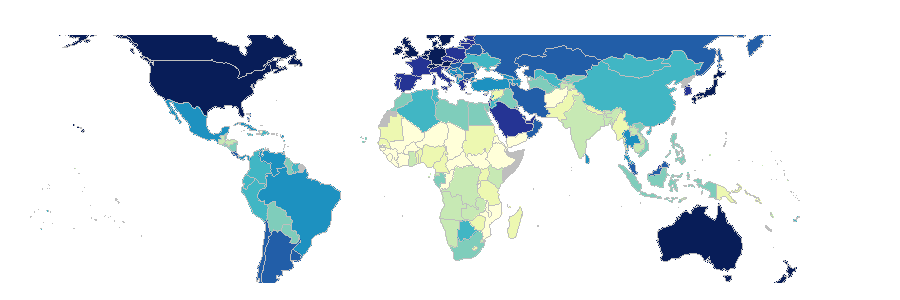
\includegraphics[width=0.9\textwidth]{world_map-HDI/world_map-HDI.pdf}
					\subcaption{Human development index by region}\label{fig:world_map-HDI}
				\end{subfigure}

				\begin{subfigure}[b]{1\textwidth}
					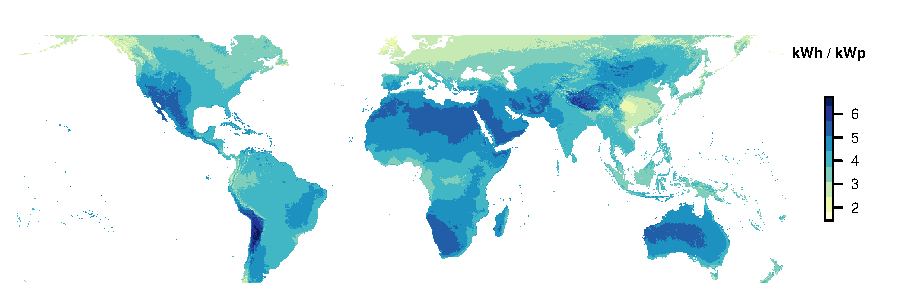
\includegraphics[width=0.9\textwidth]{world_map-PVOUT/world_map-PVOUT.pdf}
					\subcaption{Daily photovoltaic electricity potential}\label{fig:world_map-PVOUT}
				\end{subfigure}

				\begin{subfigure}[b]{1\textwidth}
					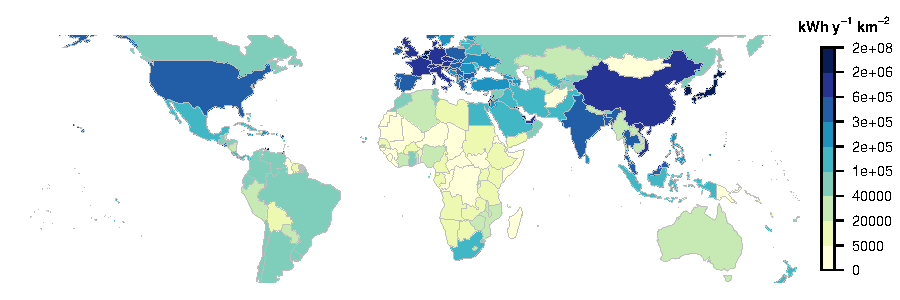
\includegraphics[width=0.9\textwidth]{world_map-electrical_vs_land/world_map-electrical_vs_land.pdf}
					\subcaption{Yearly electricity consumption over region land area}\label{fig:world_map-electrical_vs_land}
				\end{subfigure}
				\mycaption[Geographical distribution of development, sunlight and consumption.]{Data in (\textbf{a}) represent the human development index:
					"a summary measure of average achievement in key dimensions of human development: a long and healthy life, being knowledgeable and have a decent standard of living"
					from UNDP\cite{UNDP2018} (missing data in grey); data in (\textbf{b}) represents the photovoltaic electricity potential: considering a photovoltaic module installed in a region, is the ratio between the average daily produced energy, in kWh, and the nominal power, or nameplate capacity, of the installed module;\cite{Solargis2018} data in (\textbf{c}) represents the yearly electricity consumption\cite{CIAa} (comparing total electricity generated annually plus imports and minus exports) on a country scale divided by country land surface,\cite{CIA} expressed in kilowatt-hour per year and per square kilometre.}\label{fig:world_map}
			}}
	\end{figure}

	\paragraph{Resilience}
	The usage of photovoltaic energy source is compatible with a distributed and decentralized network model.
	Such a power network can be much more resilient than the fossil fuels based system, with the only single-point-of-failure being the climate variability.
	%	is the electric energy production method that best matches a distributed and decentralized network model, 
	Combined with accumulation (needed for night time usage) and with other energy sources, it can be the pivot of an extremely reliable electric energy provisioning system.

	\paragraph{More energy is not enough} It is intuitive that increasing the energy production is a high-price solution to the growing energetic demand.
	Indeed, in some regions a decrease in the electricity consumption has to be included for a long-term solution.
	For example, a study\cite{Margolis2016} reports that if every rooftop (not considering utility-scale solar facilities) in United States of America was covered with solar panel, just the 39~\% of its nowadays national consumption would be covered.
	In \cref{fig:world_map-electrical_vs_land} we can see how electricity consumption density is greatly inhomogeneous and comparing with the photovoltaic potential map in \cref{fig:world_map-PVOUT}, it is evident that such a problem is shared with many other poorly insulated but energy eager regions.
	Both an increase in machinery's efficiency and a change in life-style can be part of the solution, following the example and thinking at life-style, in USA the \textsl{per capita} energy usage is more than twice the European average, and five times the Latin America average.\cite{IEA}

	\paragraph{And more research is needed} Every source of electrical energy we can think of works \textsl{via} the conversion of motive power (a flow of steam, wind, or water, waves, tides...) to electricity, which relays on the well established electric generator.
	Except photovoltaic energy.
	This very simple difference already hints for the huge conceptual and technological step required by photovoltaics as compared to other electrical energy sources.

	% transducer
	\mysection[Relevant Physics]{Relevant Physics for Stacked Semiconductor Thin Films}

	\subsection{Energy Levels and Occupancy}
			
	\begin{SCfigure}
		\centering
		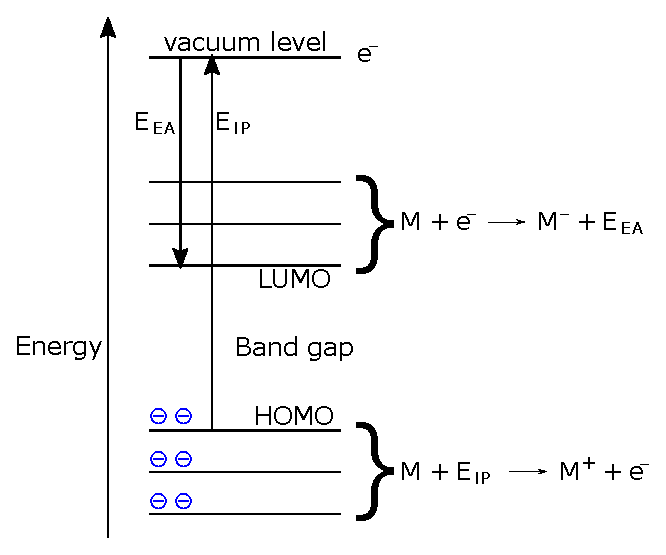
\includegraphics[width=0.7\textwidth]{homo_lumo/homo_lumo.pdf}
		\mycaption[Representation of HOMO and LUMO levels.]{See description in the text.
		}\label{fig:homo_lumo}
	\end{SCfigure}
		
		\paragraph{HOMO and LUMO}
		The energy that an electron can have when it is bound in a nanometric volume (like a molecular bond) is quantized, the possible energies are represented in \cref{fig:homo_lumo}.
		The lowest levels represent the ones filled with electrons and their energy is defined as the energy that can be provided to a neutral isolated molecule at its ground state which result in one electron being separated from it at an infinite distance.
		The minimum of these ionization energies, is the \gls{homo}.
		The highest levels are virtual ones and represent the energies that can be gained when an unbound electron gets bound to a isolated molecule which was neutral and at its ground state.
		The maximum of these electron affinity energies, is the \gls{lumo}.
		The difference between \gls{homo} and \gls{lumo} is named band gap.
		After these processes, the molecule will geometrically change and release some reorganization energy, but this is not included in the \gls{homo} and \gls{lumo} definition (\textsl{i.e.} a vertical transition is considered).
		

		\paragraph{Valence and conduction bands}
		

		\paragraph{Boltzmann and Fermi-Dirac statistics}

		\paragraph{Fermi and quasi-Fermi levels}

	\subsection{Electrostatics}

		\paragraph{Poisson equation}

		\paragraph{Space charge limited layers, Debye length and electric field screening}\label{intro-space_charge}
		\cite{WikipediaDebye2019}

	\subsection{Electrodynamics}

		\paragraph{Charge diffusion}

		\paragraph{Charge drift}

		\paragraph{Displacement current -- definition}\label{intro_displacement_current} The displacement current $J_D$ appears in the fourth macroscopic Maxwell's equation as $\partial D / \partial t$ for describing the contributions to magnetizing field not originated by a current of free charges $J_f$: $\nabla \times H = J_f + \frac{\partial D}{\partial t}$.
		The displacement electric field $D$ includes contributions from the electric field intensity $E$ and the polarization $P$: $D=\epsilon_0 E + P$ which can also be written in terms of relative permittivity $\epsilon_r$ as: $D= \epsilon_0 \epsilon_r E$.
		So its time derivative defining the displacement current is: $\frac{\partial D}{\partial t} = \epsilon_0 (\epsilon_r\frac{\partial E}{\partial t} + E\frac{\partial \epsilon_r}{\partial t})$.
		For the scope of this thesis we're interested in the first term and we're going to ignore the second one considering the relative permittivity as a material dependent constant.


		\begin{figure}
			\makebox[\textwidth][c]{
				\parbox{1.1\textwidth}{
					\centering
					\begin{subfigure}[t]{0.5\textwidth}
						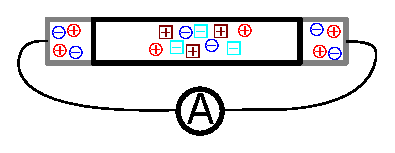
\includegraphics[width=1\textwidth]{displacement_current/first.pdf}
						\subcaption{Initial condition}\label{fig:displacement_current-initial}
					\end{subfigure}
					\bigskip

					\begin{subfigure}[t]{0.5\textwidth}
						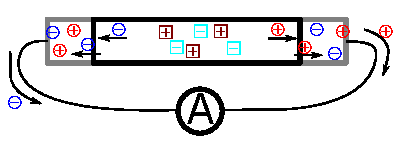
\includegraphics[width=1\textwidth]{displacement_current/second.pdf}
						\subcaption{Free charges crossing interfaces}\label{fig:displacement_current-electronic}
					\end{subfigure}
					\qquad
					\begin{subfigure}[t]{0.5\textwidth}
						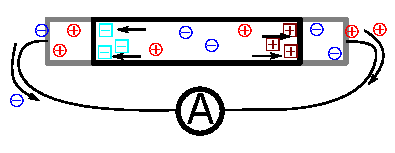
\includegraphics[width=1\textwidth]{displacement_current/third.pdf}
						\subcaption{Ions accumulating at interfaces}\label{fig:displacement_current-ionic}
					\end{subfigure}

					\mycaption[Representation of current and displacement current.]{(\textbf{a}) a mixed ionic-electronic conductor material layered between two layers of electronic conductor material.
						(\textbf{b}) the electronic charge can cross the material's interfaces.
						(\textbf{c}) ionic charge cannot be transferred to the electrodes, still a displacement current due to the ionic migration is generated and can be measured in the amperometer.}\label{fig:displacement_current}
				}
			}
		\end{figure}


		\paragraph{Displacement current -- interpretation} So the displacement current accounts for the charge movements not identifiable as current and for their effect on the surrounding circuitry.
		An example is represented in \cref{fig:displacement_current-ionic}: the amperometer can measure a current even if no charge crossed the perovskite/electrode interface, this is a displacement current caused by the creation of a dipole due to the ionic accumulation at the interfaces.
		One can imagine the resulting current as needed for maintaining the zero potential difference between the two contacts.
		It is not, as one could erroneously and instinctively think, the effect of an electric field generated in the contacts by the moving charge in the perovskite layer (with related Coulomb force and image charges) as out of the two two-dimensional planes of opposed charges no electric field is present.
		This can be understood thinking that the electric field intensity generated by a large plate of charges has a constant magnitude at distances much smaller than the plate dimensions (which is always true in our solar cells considering the thickness \SI{\approx 1}{\um} to area \SI{3x3}{\square\mm} ratio, except at electrode edges).
		The concept is represented in \cref{fig:dipole_plane}.
		In \cpageref{displacement_current_ionic} we'll use the displacement current concept for simulating the current caused in the electrodes not by a net flux of charges through a device section but by the rearrangement of charges which not necessarily leave the device, like the ionic migration in perovskite material.

		\begin{figure}
			\makebox[\textwidth][c]{
				\parbox{1.1\textwidth}{
					\centering
					\begin{subfigure}[t]{0.41\textwidth}	\centering
						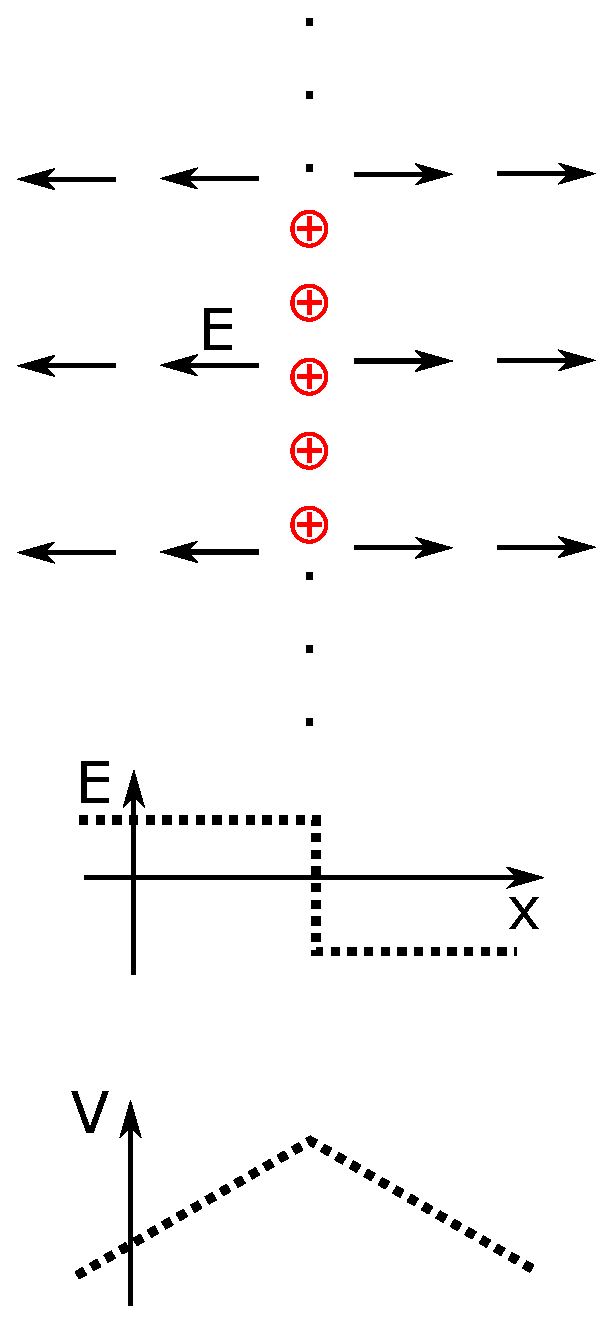
\includegraphics[height=0.3\textheight]{dipole_plane/single.pdf}
						\subcaption{Infinite plane of charges}\label{fig:dipole_plane-single}
					\end{subfigure}
					\qquad
					\begin{subfigure}[t]{0.61\textwidth}	\centering
						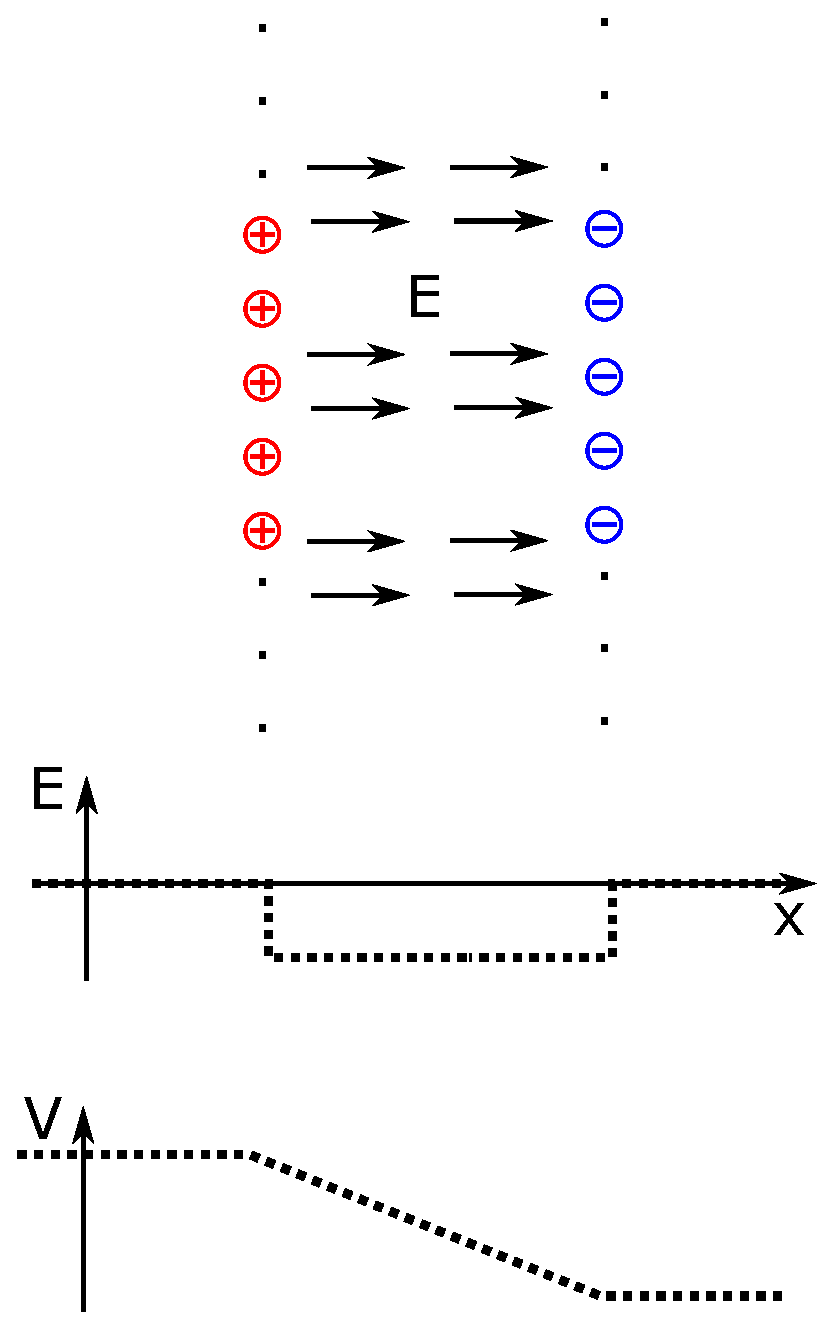
\includegraphics[height=0.3\textheight]{dipole_plane/double.pdf}
						\subcaption{Two infinite planes of opposed charges}\label{fig:dipole_plane-double}
					\end{subfigure}

					\mycaption[Electric field by two planes of opposite charges.]{(\textbf{a}) an infinite plane of charged particles is represented, the electric field is constant on the two sides, with a discontinuity in the plane.
						(\textbf{b}) adding a second plane with the same concentration of charges of the opposite kind, the electric field out of the sandwich cancels out.
						What is present outside of the sandwich is just an electrostatic potential difference.}\label{fig:dipole_plane}
				}
			}
		\end{figure}

		\paragraph{Continuity equations} The continuity equations have a very intuitive meaning: the concentration of a specie in a specific volume can increase due to generation $G$, can decrease due to recombination $U$ or can change due to a speed change of a charge flow passing by.
		This last contribution can be understood with the following example: a traffic light stops the cars flow and causes the increase of their concentration.
		For electron concentration $n$:
		\begin{equation}
			\frac{\partial n_x}{\partial t} = \frac{1}{q}\nabla_x \cdot J_n + G_{n,x} - U_{n,x}
		\end{equation}



	\subsection{Charge Recombination}

		\paragraph{Primary geminate recombination} \label{intro_geminate} This kind of recombination happens with the annihilation of a photo-generated exciton prior to the free charges separation.
		This is independent from the illumination intensity, so it can be considered as having a reaction order of zero.
		Lead halide perovskite have quite a high static permittivity \cite{Moia2019} and a small electron effective mass (high free carriers mobility) \cite{Herz2017}, this means that, at room temperature, the exciton binding energy is even smaller than $k_|B|T$ \cite{Miyata2015,Galkowski2016,Tvingstedt2015} and the direct generation of free charges occurs.
		So this kind of recombination is negligible in perovskite solar cells CITATION NEEDED.
		%Non-geminate recombination refers to the annihilation of an electron and an hole happening after their complete separation, as opposed to geminate recombination where the recombination happens just after the charges separation but before their distancing.

		\paragraph{Radiative recombination}
		This is an unavoidable form of recombination, which finds its origin in the detailed balance principle describing that, at steady state, all the absorbed thermal photons, coming from the surroundings of the cell, have to be re-emitted as black body radiation.
		From this parallelism it can be understood that this recombination is larger for materials with greater absorptivity \cite{Nelson2003} like the ones used for thin film solar cells \cite{Tvingstedt2015}.
		An indirect bandgap disfavours the radiative recombination: in these materials the recombination involves a large momentum variation, while the photon emitted due to the recombination can take just a small momentum and the rest of it should be released as an additional phonon (lattice vibrations).
		Radiative recombination involves the collision of two opposite free charges, so it can be considered as having a reaction order of 2 when electrons and holes concentrations are similar, $n \approx p$ (in intrinsic semiconductors out of the depletion layer or, in intrinsic perovskites, once ionic profile stabilized cancelling the electric field), while in case of uneven concentrations (in doped semiconductors or inside depletion layers) the limiting reagent is the minority carrier (electrons in p-type and holes in n-type materials) and the reaction order is 1.
		The expression used for modelling is: $U_|rad| = k_|rad| (np-n_|i|^2)$, where $n_|i|$ is the intrinsic carrier density as obtained from Boltzmann distribution for an intrinsic semiconductor, it is just introduced in the equation in order to account for the thermal generation.
		This type of recombination is present in perovskite solar cells, indeed some of the most efficient perovskite solar cells can be used as \gls{led} taking advantage of their radiative recombination \cite{Bi2016}.

		\paragraph{SRH trap mediated recombination}
		Also known as Shockley-Read-Hall recombination \cite{Shockley1952}, this recombination happens in two steps: a free charge from the respective band decays into an empty localized state with energy in between the valence and the conduction bands, a trap, after this event, a free charge of the opposite sign reaches the trapped charge location and recombine with it.
		As aforementioned, in an indirect band gap material the radiative recombination is disfavoured, but the presence of a trap state can divide in two easier steps the charge recombination process.
		%		In an indirect band gap material (where the momentum difference between the starting and final state is large) band-to-band bimolecular radiative recombination is disfavoured, but the presence of a localized trap state can catalyse the transition 
		Usually both the momentum difference and the chemical energy is released \textsl{via} phonons, so no radiative emission is involved.
		This recombination type can have reaction order of 1 or 2 depending on how many of these steps constitutes a bottleneck \cite{Calado2018b}.
		In case of mid-gap traps (with energy in the middle of the bandgap), these states will be rather saturated and the process of trapping a free charge will be slow as an empty trap has to be hit, then the actual recombination is fast, so the reaction order is 1.
		In case of shallow traps, the first step could or could not be a bottleneck, this time depending on the availability of free charges to trap: in doped semiconductors this could be a limiting factor, and the reaction order would be again 1; in intrinsic semiconductors there will be plenty of free charges of both types, and the reaction order can get close to 2.
		The expression used for modelling is \cite{Shockley1952}:
		\begin{equation}\label{eq:srh}
			U_{SRH} = k_{SRH} \frac{np-n_|i|^2}{\tau_n(p+p_t)+ \tau_p(n+n_t)}
		\end{equation}
		where $n_t$ and $p_t$ AAAAAAAAAAAAAAAAAAAAAAAAAAAAAAAAAAAAAAAA
		For lead halide hybrid perovskite materials, this kind of recombination is or is not important depending on the presence of mid-gap states, which in turn depends on the material composition and stoichiometry CITATION NEEDED.

		\paragraph{Surface recombination}\label{intro_surface_recombination}
		Also known as interfacial recombination, refers to the annihilation of one kind of free charge on a material with a charge of the opposite sign located on another material, happening at the materials' interface.
		At the interface between a, for example, p-doped and a close-to-intrinsic material as we consider the perovskite, the surface recombination will involve the majority carrier, holes, in the doped material and the opposite charge in the intrinsic semiconductor.
		As the doped semiconductor has abundance of majority carriers, the limiting factor will be the concentration of "minority" carriers on the other side of the interface, which will depend on its mobility and on the electric field in the intrinsic.
		So the reaction order should be 1 for this case.
		The presence of mid-gap states in the doped selective contact can mediate the recombination in a fashion similar to the aforementioned Shockley-Read-Hall mechanism.
		In efficient perovskite solar cells, this is the most important recombination pathway CITATION NEEDED.

		\paragraph{Auger recombination}
		When a free charge gets in contact with another of the same kind, it is possible that one of these decays and the other absorbs the just released energy as kinetic energy.
		Additionally to the two free charges of the same kind, it also requires a free charge of the opposite kind for the decay to be possible, so it can be considered as having a reaction order of three.
		This recombination is important in materials with high free carriers densities or at high photo-generation conditions.
		These high charge densities are unlikely to happen in perovskite solar cells at normal working conditions.

	\subsection{Charge Generation}

		\paragraph{Light absorption}

		\paragraph{Light absorption in presence of electric field}\label{intro_electroabsorbance}

		\paragraph{Excitons and free charges generation}

	\subsection{PhotoVoltaic Effect}

		\paragraph{Charge collection}

		\paragraph{Electromotive force}

		%https://en.wikipedia.org/wiki/Electromotive_force#Solar_cell

\section{Perovskite Solar Cells}
	\epigraph{\textit{\enquote{That's yogurt science!}}}

	Perovskite solar cells is a relatively new player in the photovoltaics world, existing just since 2009 (started by the research groups Miyasaka \cite{Kojima2009}, Park \cite{Im2011a,Kim2012b}, and Snaith \cite{Lee2012}).
	This type of solar cells evolved from the \gls{dssc} tradition, where an absorber dye is in contact with a titania \gls{etm} and an organic \gls{htm}.
	Here the absorber dye is substituted by a hybrid organic-inorganic lead halide perovskite semiconductor and both the \gls{etm} and the \gls{htm} can be composed of various, either organic or inorganic, materials.
	Thanks to the enormous research effort, these kind of devices reached a record stabilized efficiency of 20.9~\% \cite{Green2019} with reports of even higher non-stabilized efficiencies (23.7~\% \cite{Green2019,Jiang2017}); all this in relatively short time as represented in \cref{fig:nrel_chart}.




	\begin{SCfigure}
		\centering
		\includegraphics[width=0.5\textwidth]{nrel_chart/pv-efficiencies-2019-01-03.pdf}
		\mycaption[NREL chart of "Best Research-Cell Efficiencies"]{Just the perovskite solar cells (not stabilized) results have been reported.}\label{fig:nrel_chart}
	\end{SCfigure}

	\paragraph{Composition}

	Cesium introduction \cite{Bi2016,Saliba2016}


\begin{figure}
	\makebox[\textwidth][c]{
		\parbox{1.1\textwidth}{
			\centering
			\begin{subfigure}[t]{0.45\textwidth}
				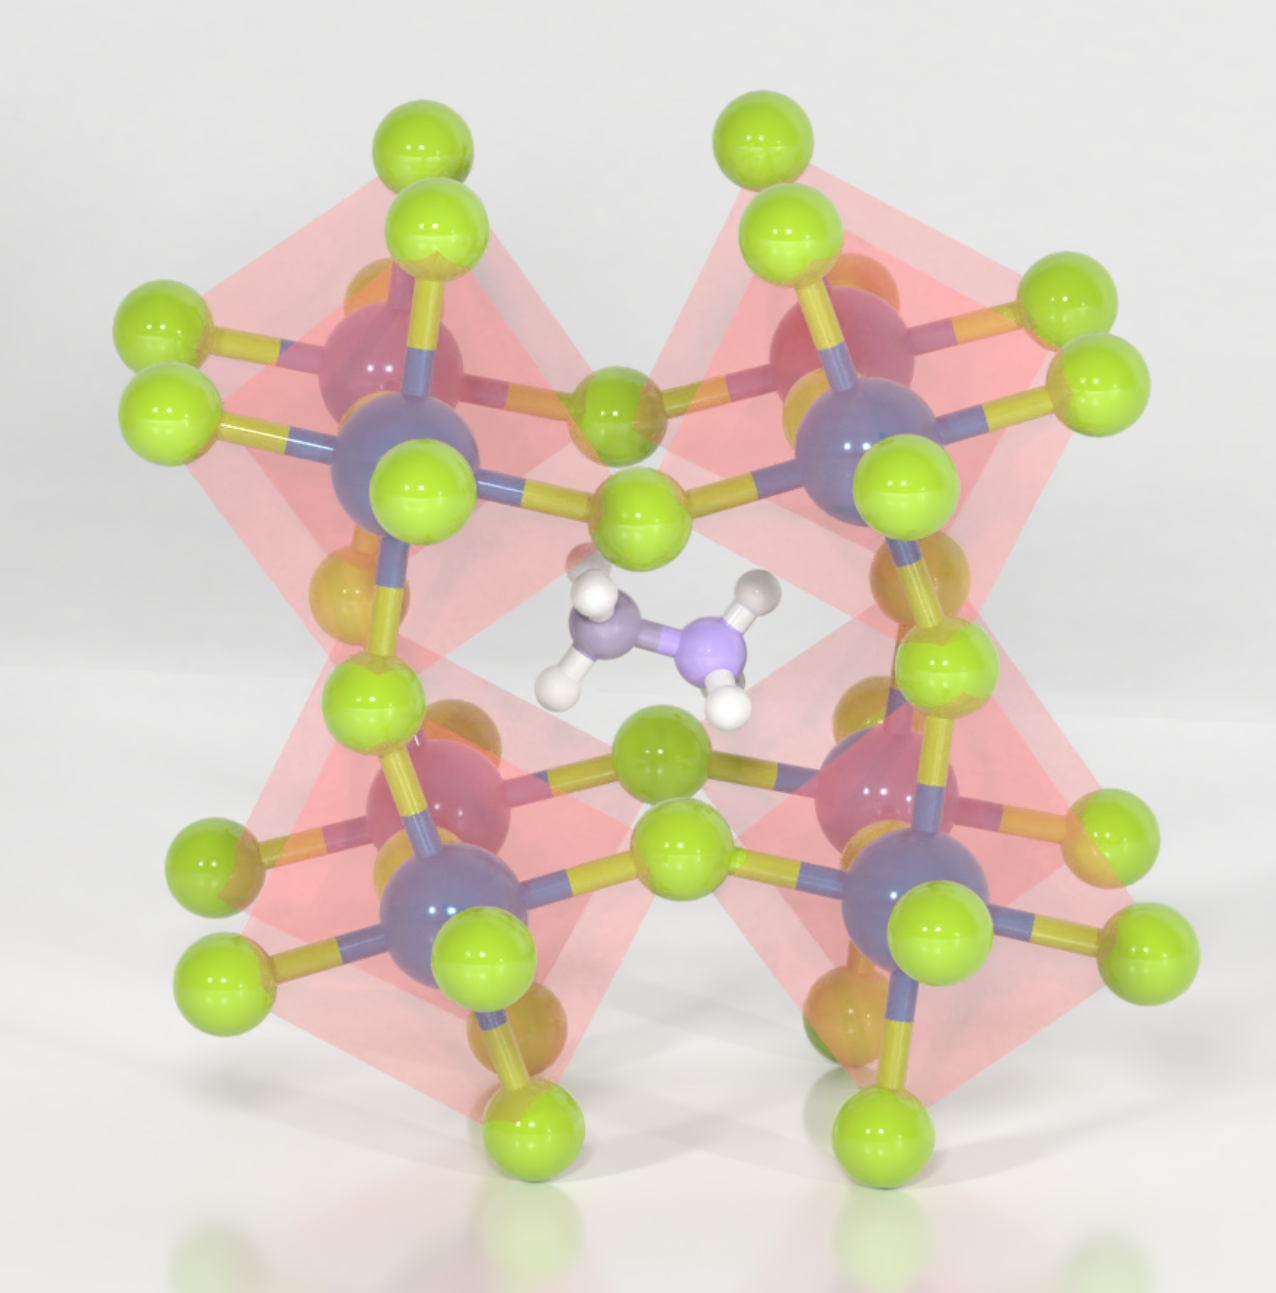
\includegraphics[width=1\textwidth]{crystal_perovskite_edvin_fako/ilario2-crop.jpg}
				\subcaption{}\label{fig:crystal-single}
			\end{subfigure}
			\qquad
			\begin{subfigure}[t]{0.57\textwidth}
				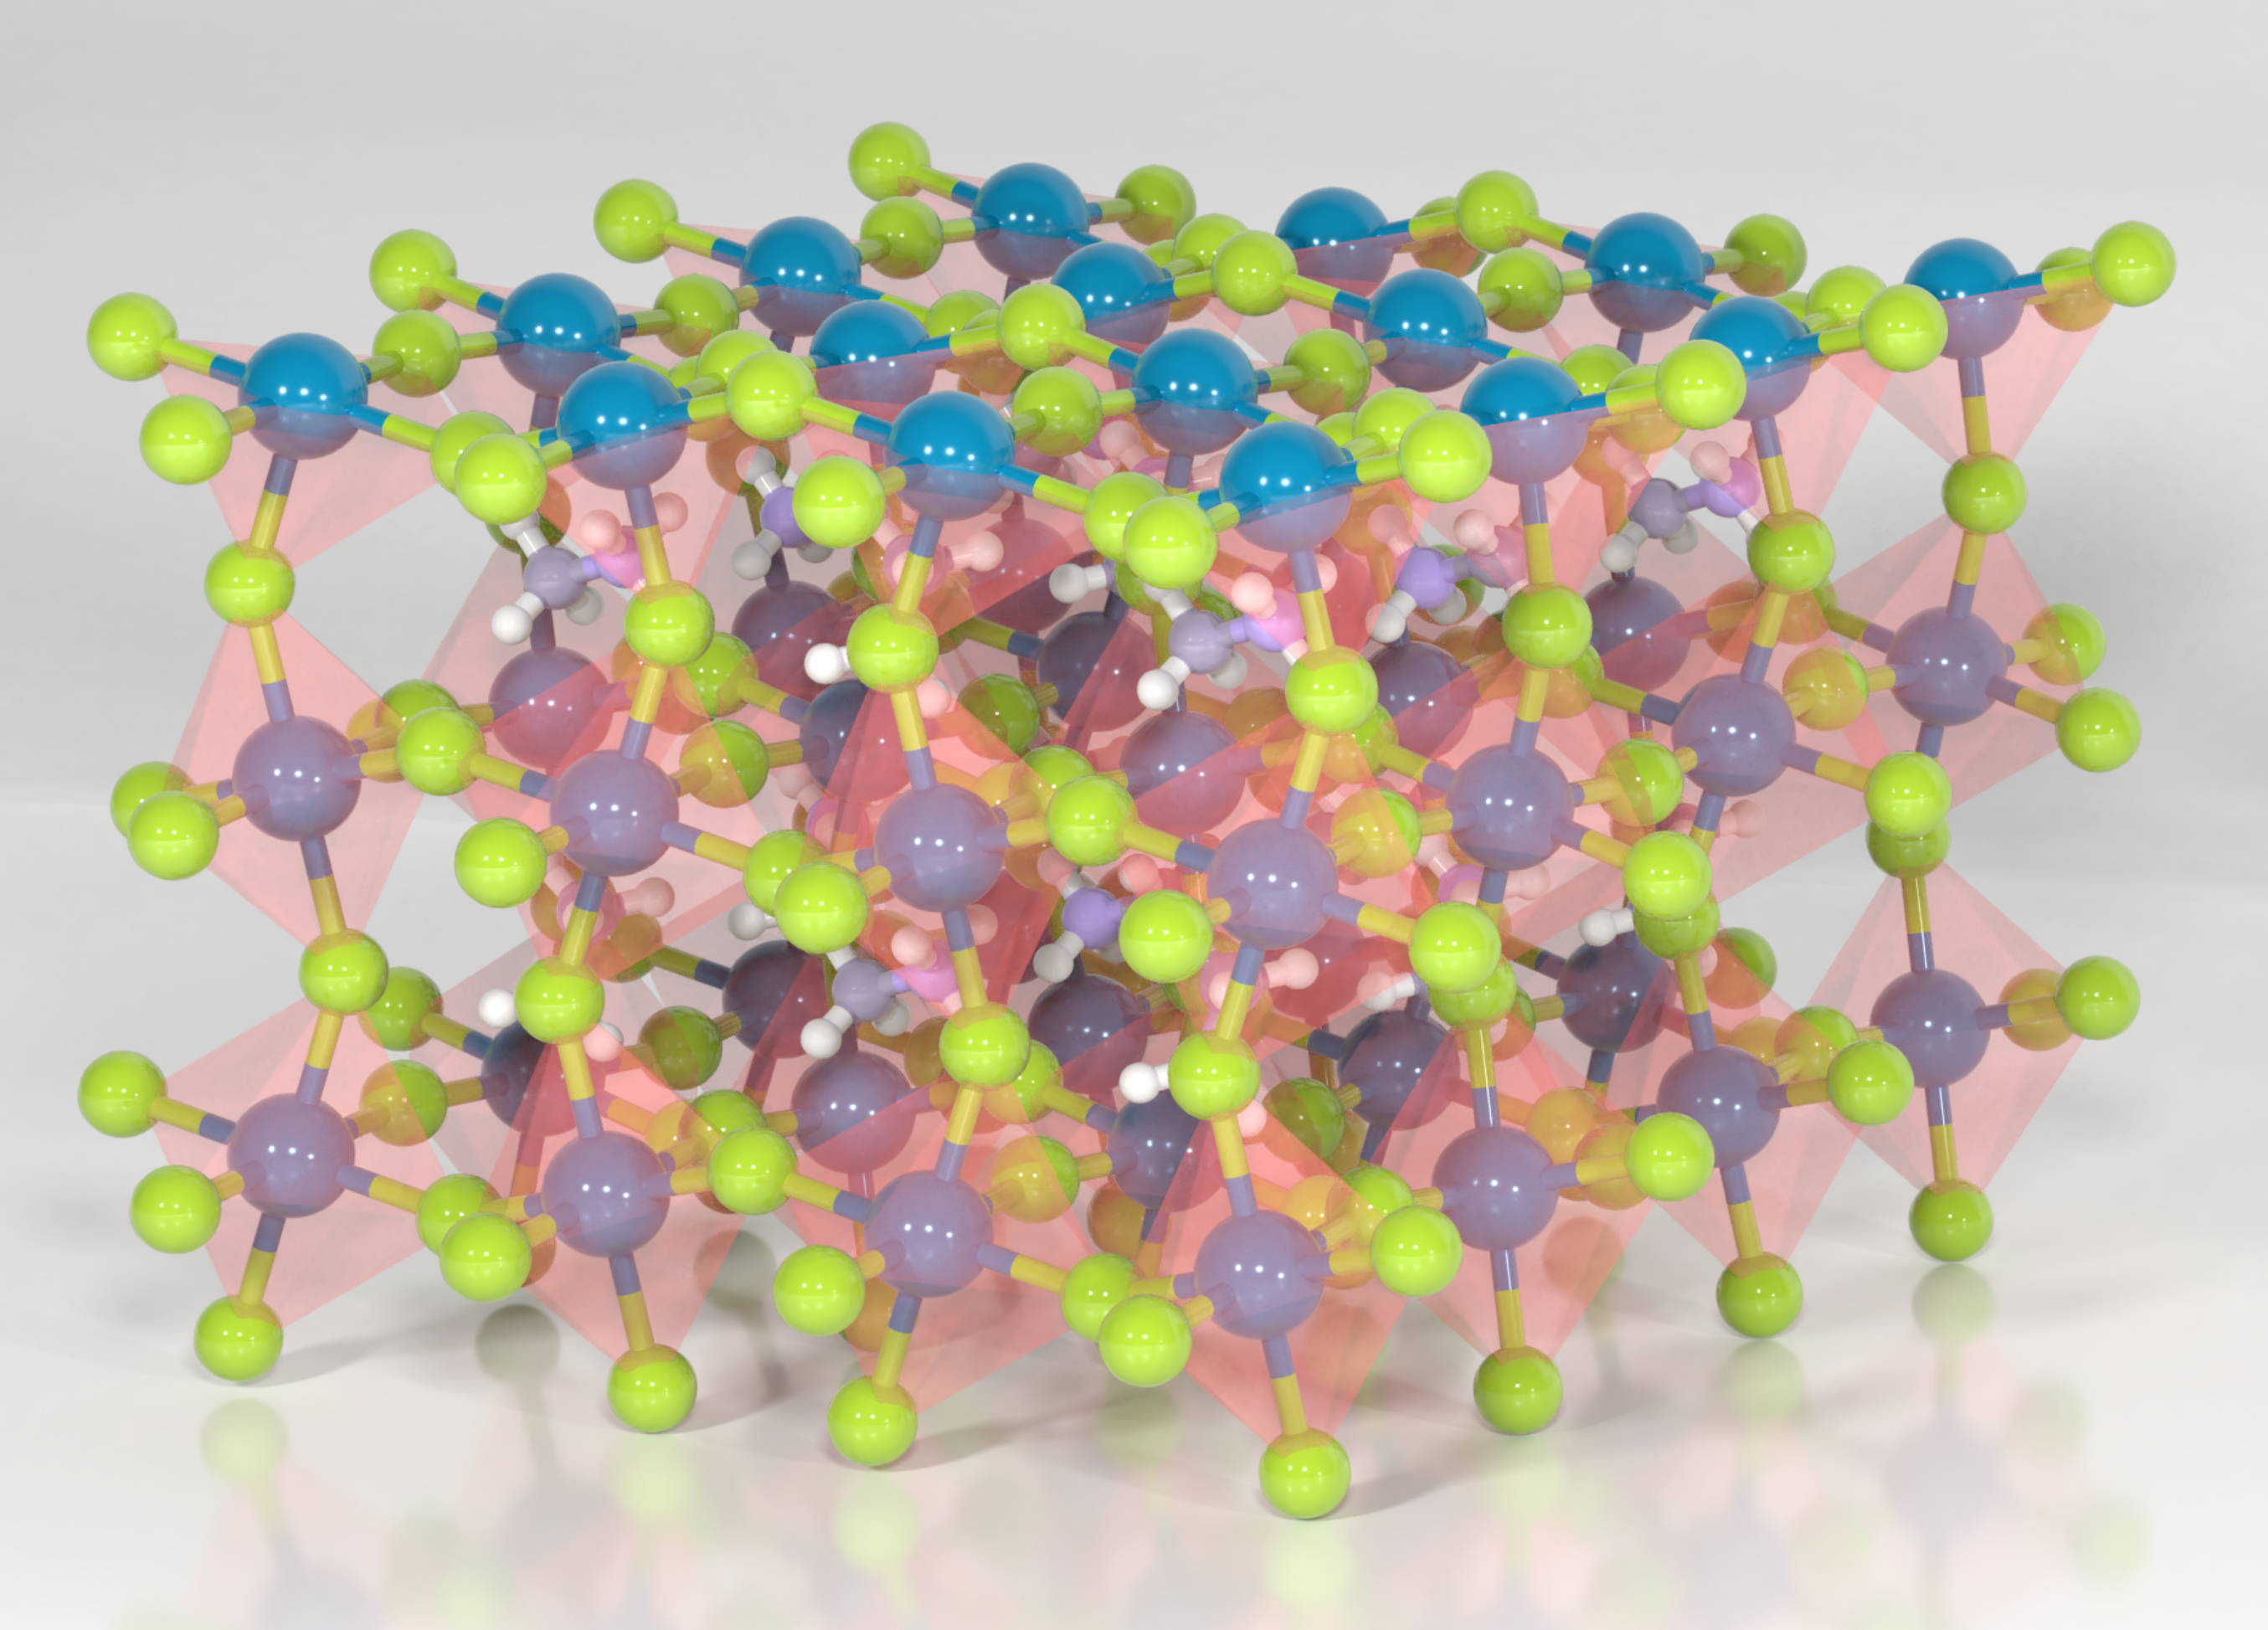
\includegraphics[width=1\textwidth]{crystal_perovskite_edvin_fako/ilario1-crop.jpg}
				\subcaption{}\label{fig:crystal-bulk}
			\end{subfigure}
			\mycaption[Crystal structure of \glsentrytext{mapi} perovskite.]{In (\textbf{a}) the methylammonium cation is between \ch{PbI6} octahedra.
			In (\textbf{b}) the bulk structure is represented.
		These graphics, created with Vasp and Blender software, are courtesy of Edvin Fako \texttt{<efako@iciq.es>}.
	}\label{fig:crystal}
		}
	}
\end{figure}


	\paragraph{Perovskite Absorber Synthesis}
	The preparation of this hybrid semiconductor \textsl{via} spin coating and annealing at low temperature is extremely easy and convenient for small-scale research purposes.
	%	From my point of view, 
	Nevertheless, this fabrication process is affected by a low reproducibility, likely due to the sensibility of the drying and crystallization step \cite{Pockett2015}.
	This factor clearly slows down the research in perovskite solar cells.
	In literature various reports of completely different results obtained from supposedly identical synthesis can be found \cite{Pockett2015,Gottesman2014}.
	This issue is being addressed recently with the publication of more reliable and complete fabrication procedures \cite{Saliba2018}.

	\paragraph{Recombination mechanisms}\label{intro_prv_recombination}
	The non-radiative recombination inside the perovskite material is surprisingly low for a low temperature processed material.
	This is demonstrated by the large diffusion length in isolated crystals \cite{Wehrenfennig2014,Wehrenfennig2014a,Stranks2013,Xing2013,Shi2015a,Eperon2014}: for the \gls{csfamapbibr} it is reported being \SI{\approx140}{\nm} for the electrons and \SI{\approx1.9}{\um} for holes \cite{Liu2017}.
	This is confirmed by the fact that once a thin layer (\SI{\approx500}{\nm}) of the material is layered between an \gls{etm} and an \gls{htm} the photoluminescence lifetime is dramatically reduced \cite{Jimenez-Lopez2017,Eperon2014} indicating that the free charges can diffuse at least over the layer thickness.
	Even if not always the case \cite{Valadez-Villalobos2019,Tress2018}, it is often reported that at open circuit conditions, the predominant recombination pathway in perovskite solar cells is identifiable as the surface recombination at the perovskite/selective contacts interfaces \cite{Calado2018b,Stolterfoht2018a,Stolterfoht2018,Gelmetti2019,Shao2016,Correa-Baena2017,Hou2016}.
	%	Considering the perovskite material, traps are more likely to form on the surface of crystal domains, where the bulk symmetry is broken and carrier-phonon coupling, which can ease indirect transitions is more likely due to the easier deformation of the broken structure . 
	Nevertheless, also the morphology and composition of perovskite material can have an impact on the \gls{voc}: non-passivated perovskite surface states which can act as traps \cite{Zheng2017} thanks to the easier deformation of the broken crystal cell, favouring the electron-phonon coupling needed for indirect transitions \cite{Wu2015}; inhomogeneous perovskite layer can lead to pinholes \cite{Lee2015,Montcada2017,Qiu2016}; accessible grain boundaries due to non-compact perovskite layer causes the presence of more recombination centres \cite{Shao2016a}; the presence of secondary phases with in-gap energies can be reduced modifying the perovskite composition \cite{Bi2016}.

	\paragraph{Open circuit voltage}
	The open circuit voltage of a perovskite solar cell depends on many contributions.
	As we will see in \cref{ch:characterization}, the aforementioned charge recombination rate is one of these.
	This recombination is more important in a perovskite solar cell rather than in \gls{osc} as the built-in field is shielded by the ionic accumulation and the minority carriers concentration at the perovskite\-/contacts interfaces is higher.
	A contact material having mid-gap states will favour the surface recombination, but also its additives (\textsl{e.g.} dopants, dispersants\dots) can introduce such trap states \cite{Correa-Baena2017}.
	Additionally, a different material employed as \gls{etm} and \gls{htm} will result in a different built-in voltage (difference in contacts' Fermi levels energies), which is often regarded as a limit for the the open circuit voltage \cite{Gelmetti2019,Wu2016}.
	The presence of ionic accumulation in perovskite solar cells have been reported to reduce the influence of the \gls{voc} from the built-in voltage \cite{Belisle2016}.
	Even a different molecular ordering in the selective contacts can influence the \gls{voc} through the variation of the \gls{dos} width, and by consequence the energetics of the band edges \cite{Shao2016}.
	Rather than a hard limit, the built-in voltage represents the applied voltage that saturates the depletion layers in the contacts, which implies a large charge density at the materials interface and an important surface recombination CITATION NEEDED.
	Indeed, it has been shown that suppressing the surface recombination can allow a device to give a voltage higher than the built-in voltage. CITATION NEEDED
	A large absorber band gap will have the excited charges thermally relaxing to a more energetic band, allowing the solar cell to achieve a higher \gls{voc}.
	The perovskite band gap can be easily tuned changing its stoichiometry, for example partially replacing iodine with bromine \cite{McMeekin2016,Noh2013a,Wheeler2017} or using different organic cations \cite{Eperon2014}.
	For perovskite solar cells, the record reported \textit{bandgap\hyp{}voltage offset} are already much smaller than the voltage losses reported for \gls{osc} \cite{Tvingstedt2015}.
	If we consider the possibility of having the injection of hot carriers (free charges generated by a photon with energy larger than the band gap) into the contacts before their thermal relaxation to the band edge, also a \gls{voc} larger than the absorber band gap is possible CITATION NEEDED and could, at least theoretically, make possible to break the Shockley\hyp{}Queisser limit \cite{WikipediaSQlimit}.

	\paragraph{Charge extraction and charge blocking}
	Selective contacts are in charge of selectively extract one kind of charge, blocking the other.
	Clearly, the relative position of the perovskite and selective contact energy level is key both for extraction \cite{CorreaBaena2015} and for blockage CITE SOMETHING.

	\paragraph{Ionic migration}
	Ionic conductivity in halide perovskite materials has been pointed out more than 35 years \cite{Mizusaki1983,Yamada1995,Yamada1998}.
	More recently, the presence of mobile ionic species has been confirmed also for hybrid lead halide perovskites, using \gls{kpfm} \cite{Birkhold2018},  XXXXXXXXXXXXXXXXXX
	%	The presence of and mobile ionic species have been demonstrated in various kind of hybrid lead halide perovskite materials.
	In complete perovskite solar cells, it has been observed even for devices not showing any current-voltage hysteretic behaviour \cite{Calado2016,Jacobs2018,Bryant2015}.
	For \gls{mapi} perovskite, the majoritarian mobile species has been identified as iodine vacancy XXXXXXXXXXXXXXXX \cite{Yang2015e,Senocrate2017} while a significant contribution from methylammonium ions migration has been excluded \cite{Senocrate2018,Senocrate2017}.
	These charged species can migrate inside the material either by diffusion or when drifted by an electric field \cite{Xiao2015}.

	\paragraph{Field free absorber}
	Thanks to the abundance of the ionic specie CITATION, the free charge concentration is low \cite{Walsh2015} and the electric field inside the absorber is completely shielded \cite{Tress2015}.

	diffusive transport vs drift transport

	characterization complexity reduction due to more homogeneous carriers profile \cite{Kirchartz2012}

	\paragraph{Diffusion as the main transport mechanism}(due to the built-in voltage being the workfunction difference of the selective contacts)(drift is not the main transport mechanism in stabilized perovskite solar cells due to the electric screening effect of the mobile ionic species)


	\paragraph{Hysteresis}
	Hysteretic behaviour in current-voltage sweeps, while not often observed in other kind of solar cells, it is frequent in perovskite solar cells.
	Still, many reports of hysteresis-free perovskite solar cells can be found, especially for top cathode or for high performances bottom cathode devices.
	As we saw above, the presence of mobile ionic species is widely accepted for most of the hybrid lead perovskite materials and this has been indicated as one of the causes of the hysteresis \cite{Unger2014,Xiao2015}.
	Considering that the recombination and collection of free charges is affected by the ions-modulated electric field \cite{Pockett2017}, this is enough to explain the presence of hysteresis \cite{Tress2015,Calado2016} \textsl{via} the modulation of interfacial energy barriers \cite{Moia2019}.
	Additionally, adsorption or chemical reaction of perovskite ionic defects with the selective contact surface (\textsl{e.g.}\ with titanium oxide \cite{Yu2016,Beilsten-Edmands2015,Carrillo2016} or tin oxide CITATION NEEDED) could be important and can explain why \cite{Moia2019}, bottom cathode cells with inorganic contacts usually present hysteresis while top cathode with all-organic contacts usually does not.

%	\paragraph{Intrinsic or doped semiconductor}


	\paragraph{Characterization}
	The characterization techniques for perovskite solar cells and the relative interpretation evolved from the techniques and theory built around \gls{osc} and \gls{dssc} \cite{Barnes2013}.
	This pre-existing framework has been widely used in literature for perovskite solar cells by various research groups \cite{ORegan2015b,Shao2016,Gelmetti2019,Kiermasch2018,Carnie2015}.
	Unfortunately, perovskite solar cells are different enough from \gls{osc} and \gls{dssc} to doom the utility of most of these observations.
	Moreover, while an acceptable agreement between different characterization techniques was often observed in \gls{osc} \cite{Clarke2015,Maurano2011,Foertig2012} and \gls{dssc} \cite{Barnes2013}, in perovskite solar cells we often observe hard-to-explain discrepancies \cite{Kiermasch2018}.
	In the past few years, the theoretical framework has been expanded and should finally enable the perovskite community to re-interpret and re-design the solar cells characterization techniques.
	In \cref{ch:characterization} the reader can find some of the accepted concepts and some novel proposals about the interpretation of the classical characterization techniques when used on perovskite solar cells.

	\paragraph{Stability}
	The stability of the perovskite solar cells is the number one blocker to commercialization.
	Its keystone has still to be identified.
	An interesting investigation is being carried on by D.\ R.\ Ceratti and D.\ Cahen (unpublished) regarding the release of a proton by methylammonium cation when in contact with non-acidic materials, and thus leaving the perovskite crystal structure.
	This could explain the reports about the beneficial addition of acids in perovskite precursors solution, mainly by Snaith group \cite{Noel2017,Zhang2015a,Nayak2016}.


	https://www.ossila.com/pages/perovskite-solar-cell-degradation-causes


	Formation of HI in contact with water which reacts with silver 10.1039/C5TA00358J 10.1002/admi.201500195
	Reaction with other contact materials 10.1021/acsnano.5b03687

	Influence of perovskite material on Voc \cite{Wheeler2017,Eperon2014,Noh2013a}

	Influence of contacts on Voc \cite{CorreaBaena2015} WU2016A

%\section{Background and Related Work}\label{sec:background}
%
%	\subsection{Perovskite Solar Cells}
%
%	\subsection{Hole Transporting Materials}
%
%	\subsection{PhotoPhysical Studies and Techniques}
%
%	\subsection{Modelling and Relevant Physics}

\section{Motivation and Aims}\label{sec:aims}
\epigraph{\textit{\enquote{To begin with, we want everything.}}}{autistici / inventati}


The objectives of this thesis are:\nolinebreak
\begin{itemize}
	\item synthesize different kinds of lead perovskite absorbers (\textsl{e.g.} \gls{mapicl}, \gls{mapi}, \gls{famapbibr}, \gls{csfamapbibr});
	\item fabricate solar cells with different structures (\textsl{e.g.} top and bottom cathode);
	\item test different materials for selective contacts, either known (\textsl{e.g.} flat or mesoporous titania, \gls{pcbm70} or plain fullerene) or novel materials obtained \textsl{via} collaborations (\textsl{e.g.} \gls{tae1}, \gls{tae3}, \gls{tae4});
	\item optimisation of the devices fabrication in order to get close to the state of the art devices;
	\item characterisation of the prepared devices using the existing routine techniques (\textsl{e.g.} current\hyp{}voltage sweeps);
	\item characterisation using advanced small perturbation techniques;
	\item optimisation of the characterisation methods, data acquisition, and data processing;
	\item obtain information on the charge accumulation and charge dynamics from the characterisation output;
	\item model perovskite solar cells and compare the expected theoretical output with the experimental one;
	\item where the simulation matches the experiment, take advantage of the additional insight obtainable from the modelling.	
\end{itemize} 

